% Created by tikzDevice version 0.10.1 on 2018-06-19 09:38:51
% !TEX encoding = UTF-8 Unicode
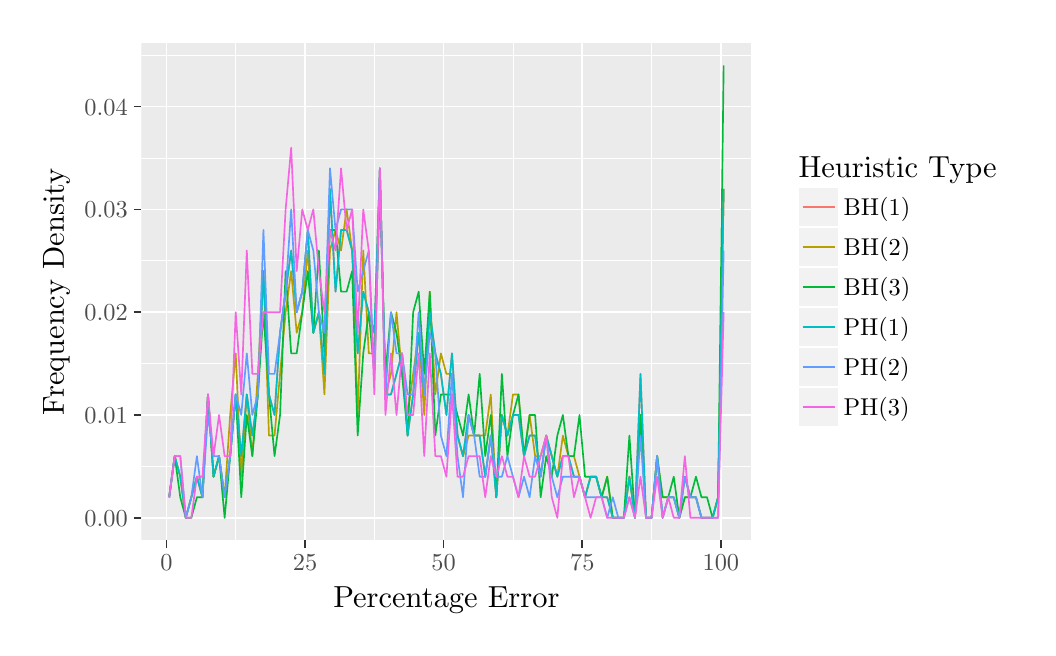
\begin{tikzpicture}[x=1pt,y=1pt]
\definecolor{fillColor}{RGB}{255,255,255}
\path[use as bounding box,fill=fillColor,fill opacity=0.00] (0,0) rectangle (361.35,216.81);
\begin{scope}
\path[clip] (  0.00,  0.00) rectangle (361.35,216.81);
\definecolor{drawColor}{RGB}{255,255,255}
\definecolor{fillColor}{RGB}{255,255,255}

\path[draw=drawColor,line width= 0.6pt,line join=round,line cap=round,fill=fillColor] (  0.00,  0.00) rectangle (361.35,216.81);
\end{scope}
\begin{scope}
\path[clip] ( 41.11, 31.53) rectangle (261.51,211.31);
\definecolor{fillColor}{gray}{0.92}

\path[fill=fillColor] ( 41.11, 31.53) rectangle (261.51,211.31);
\definecolor{drawColor}{RGB}{255,255,255}

\path[draw=drawColor,line width= 0.3pt,line join=round] ( 41.11, 58.27) --
	(261.51, 58.27);

\path[draw=drawColor,line width= 0.3pt,line join=round] ( 41.11, 95.42) --
	(261.51, 95.42);

\path[draw=drawColor,line width= 0.3pt,line join=round] ( 41.11,132.56) --
	(261.51,132.56);

\path[draw=drawColor,line width= 0.3pt,line join=round] ( 41.11,169.71) --
	(261.51,169.71);

\path[draw=drawColor,line width= 0.3pt,line join=round] ( 41.11,206.85) --
	(261.51,206.85);

\path[draw=drawColor,line width= 0.3pt,line join=round] ( 75.17, 31.53) --
	( 75.17,211.31);

\path[draw=drawColor,line width= 0.3pt,line join=round] (125.26, 31.53) --
	(125.26,211.31);

\path[draw=drawColor,line width= 0.3pt,line join=round] (175.36, 31.53) --
	(175.36,211.31);

\path[draw=drawColor,line width= 0.3pt,line join=round] (225.45, 31.53) --
	(225.45,211.31);

\path[draw=drawColor,line width= 0.6pt,line join=round] ( 41.11, 39.70) --
	(261.51, 39.70);

\path[draw=drawColor,line width= 0.6pt,line join=round] ( 41.11, 76.85) --
	(261.51, 76.85);

\path[draw=drawColor,line width= 0.6pt,line join=round] ( 41.11,113.99) --
	(261.51,113.99);

\path[draw=drawColor,line width= 0.6pt,line join=round] ( 41.11,151.14) --
	(261.51,151.14);

\path[draw=drawColor,line width= 0.6pt,line join=round] ( 41.11,188.28) --
	(261.51,188.28);

\path[draw=drawColor,line width= 0.6pt,line join=round] ( 50.13, 31.53) --
	( 50.13,211.31);

\path[draw=drawColor,line width= 0.6pt,line join=round] (100.22, 31.53) --
	(100.22,211.31);

\path[draw=drawColor,line width= 0.6pt,line join=round] (150.31, 31.53) --
	(150.31,211.31);

\path[draw=drawColor,line width= 0.6pt,line join=round] (200.40, 31.53) --
	(200.40,211.31);

\path[draw=drawColor,line width= 0.6pt,line join=round] (250.49, 31.53) --
	(250.49,211.31);
\definecolor{drawColor}{RGB}{248,118,109}

\path[draw=drawColor,line width= 0.6pt,line join=round] ( 51.13, 47.13) --
	( 53.13, 61.99) --
	( 55.14, 54.56) --
	( 57.14, 39.70) --
	( 59.14, 47.13) --
	( 61.15, 54.56) --
	( 63.15, 47.13) --
	( 65.15, 84.28) --
	( 67.16, 54.56) --
	( 69.16, 61.99) --
	( 71.17, 47.13) --
	( 73.17, 61.99) --
	( 75.17, 84.28) --
	( 77.18, 61.99) --
	( 79.18, 84.28) --
	( 81.18, 69.42) --
	( 83.19, 84.28) --
	( 85.19,128.85) --
	( 87.19, 84.28) --
	( 89.20, 76.85) --
	( 91.20,106.56) --
	( 93.21,121.42) --
	( 95.21,136.28) --
	( 97.21,113.99) --
	( 99.22,121.42) --
	(101.22,143.71) --
	(103.22,106.56) --
	(105.23,113.99) --
	(107.23, 91.70) --
	(109.24,158.56) --
	(111.24,121.42) --
	(113.24,143.71) --
	(115.25,143.71) --
	(117.25,136.28) --
	(119.25, 99.13) --
	(121.26,121.42) --
	(123.26,113.99) --
	(125.26,106.56) --
	(127.27,165.99) --
	(129.27, 84.28) --
	(131.28, 84.28) --
	(133.28, 91.70) --
	(135.28, 99.13) --
	(137.29, 69.42) --
	(139.29, 84.28) --
	(141.29,106.56) --
	(143.30, 84.28) --
	(145.30,113.99) --
	(147.30, 99.13) --
	(149.31, 91.70) --
	(151.31, 76.85) --
	(153.32, 99.13) --
	(155.32, 69.42) --
	(157.32, 61.99) --
	(159.33, 76.85) --
	(161.33, 69.42) --
	(163.33, 69.42) --
	(165.34, 54.56) --
	(167.34, 69.42) --
	(169.34, 47.13) --
	(171.35, 76.85) --
	(173.35, 69.42) --
	(175.36, 76.85) --
	(177.36, 76.85) --
	(179.36, 61.99) --
	(181.37, 69.42) --
	(183.37, 69.42) --
	(185.37, 54.56) --
	(187.38, 69.42) --
	(189.38, 61.99) --
	(191.39, 54.56) --
	(193.39, 61.99) --
	(195.39, 61.99) --
	(197.40, 54.56) --
	(199.40, 54.56) --
	(201.40, 47.13) --
	(203.41, 54.56) --
	(205.41, 54.56) --
	(207.41, 47.13) --
	(209.42, 47.13) --
	(211.42, 39.70) --
	(213.43, 39.70) --
	(215.43, 39.70) --
	(217.43, 54.56) --
	(219.44, 39.70) --
	(221.44, 91.70) --
	(223.44, 39.70) --
	(225.45, 39.70) --
	(227.45, 61.99) --
	(229.45, 39.70) --
	(231.46, 47.13) --
	(233.46, 47.13) --
	(235.47, 39.70) --
	(237.47, 54.56) --
	(239.47, 47.13) --
	(241.48, 47.13) --
	(243.48, 39.70) --
	(245.48, 39.70) --
	(247.49, 39.70) --
	(249.49, 47.13) --
	(251.49,158.56);
\definecolor{drawColor}{RGB}{183,159,0}

\path[draw=drawColor,line width= 0.6pt,line join=round] ( 51.13, 47.13) --
	( 53.13, 61.99) --
	( 55.14, 54.56) --
	( 57.14, 39.70) --
	( 59.14, 47.13) --
	( 61.15, 54.56) --
	( 63.15, 47.13) --
	( 65.15, 84.28) --
	( 67.16, 54.56) --
	( 69.16, 61.99) --
	( 71.17, 47.13) --
	( 73.17, 76.85) --
	( 75.17, 99.13) --
	( 77.18, 54.56) --
	( 79.18, 84.28) --
	( 81.18, 61.99) --
	( 83.19, 91.70) --
	( 85.19,128.85) --
	( 87.19, 69.42) --
	( 89.20, 69.42) --
	( 91.20, 91.70) --
	( 93.21,113.99) --
	( 95.21,128.85) --
	( 97.21,106.56) --
	( 99.22,113.99) --
	(101.22,136.28) --
	(103.22,106.56) --
	(105.23,113.99) --
	(107.23, 84.28) --
	(109.24,136.28) --
	(111.24,143.71) --
	(113.24,136.28) --
	(115.25,151.14) --
	(117.25,136.28) --
	(119.25, 76.85) --
	(121.26,136.28) --
	(123.26, 99.13) --
	(125.26, 99.13) --
	(127.27,165.99) --
	(129.27, 84.28) --
	(131.28, 91.70) --
	(133.28,113.99) --
	(135.28, 91.70) --
	(137.29, 76.85) --
	(139.29, 91.70) --
	(141.29,106.56) --
	(143.30, 76.85) --
	(145.30,121.42) --
	(147.30, 84.28) --
	(149.31, 99.13) --
	(151.31, 91.70) --
	(153.32, 91.70) --
	(155.32, 69.42) --
	(157.32, 61.99) --
	(159.33, 69.42) --
	(161.33, 69.42) --
	(163.33, 69.42) --
	(165.34, 69.42) --
	(167.34, 84.28) --
	(169.34, 47.13) --
	(171.35, 76.85) --
	(173.35, 69.42) --
	(175.36, 84.28) --
	(177.36, 84.28) --
	(179.36, 61.99) --
	(181.37, 76.85) --
	(183.37, 61.99) --
	(185.37, 61.99) --
	(187.38, 69.42) --
	(189.38, 61.99) --
	(191.39, 54.56) --
	(193.39, 69.42) --
	(195.39, 61.99) --
	(197.40, 61.99) --
	(199.40, 54.56) --
	(201.40, 47.13) --
	(203.41, 54.56) --
	(205.41, 54.56) --
	(207.41, 47.13) --
	(209.42, 54.56) --
	(211.42, 39.70) --
	(213.43, 39.70) --
	(215.43, 39.70) --
	(217.43, 54.56) --
	(219.44, 39.70) --
	(221.44, 76.85) --
	(223.44, 39.70) --
	(225.45, 39.70) --
	(227.45, 61.99) --
	(229.45, 47.13) --
	(231.46, 47.13) --
	(233.46, 47.13) --
	(235.47, 39.70) --
	(237.47, 47.13) --
	(239.47, 47.13) --
	(241.48, 47.13) --
	(243.48, 39.70) --
	(245.48, 39.70) --
	(247.49, 39.70) --
	(249.49, 47.13) --
	(251.49,158.56);
\definecolor{drawColor}{RGB}{0,186,56}

\path[draw=drawColor,line width= 0.6pt,line join=round] ( 51.13, 47.13) --
	( 53.13, 61.99) --
	( 55.14, 47.13) --
	( 57.14, 39.70) --
	( 59.14, 39.70) --
	( 61.15, 47.13) --
	( 63.15, 47.13) --
	( 65.15, 84.28) --
	( 67.16, 54.56) --
	( 69.16, 61.99) --
	( 71.17, 39.70) --
	( 73.17, 61.99) --
	( 75.17, 84.28) --
	( 77.18, 47.13) --
	( 79.18, 76.85) --
	( 81.18, 61.99) --
	( 83.19, 84.28) --
	( 85.19,113.99) --
	( 87.19, 84.28) --
	( 89.20, 61.99) --
	( 91.20, 76.85) --
	( 93.21,128.85) --
	( 95.21, 99.13) --
	( 97.21, 99.13) --
	( 99.22,113.99) --
	(101.22,128.85) --
	(103.22,106.56) --
	(105.23,136.28) --
	(107.23, 99.13) --
	(109.24,143.71) --
	(111.24,143.71) --
	(113.24,121.42) --
	(115.25,121.42) --
	(117.25,128.85) --
	(119.25, 69.42) --
	(121.26, 99.13) --
	(123.26,113.99) --
	(125.26, 91.70) --
	(127.27,158.56) --
	(129.27, 91.70) --
	(131.28,113.99) --
	(133.28,106.56) --
	(135.28, 91.70) --
	(137.29, 69.42) --
	(139.29,113.99) --
	(141.29,121.42) --
	(143.30, 91.70) --
	(145.30,121.42) --
	(147.30, 69.42) --
	(149.31, 84.28) --
	(151.31, 84.28) --
	(153.32, 84.28) --
	(155.32, 76.85) --
	(157.32, 69.42) --
	(159.33, 84.28) --
	(161.33, 69.42) --
	(163.33, 91.70) --
	(165.34, 61.99) --
	(167.34, 76.85) --
	(169.34, 47.13) --
	(171.35, 91.70) --
	(173.35, 61.99) --
	(175.36, 76.85) --
	(177.36, 84.28) --
	(179.36, 61.99) --
	(181.37, 76.85) --
	(183.37, 76.85) --
	(185.37, 47.13) --
	(187.38, 61.99) --
	(189.38, 54.56) --
	(191.39, 69.42) --
	(193.39, 76.85) --
	(195.39, 61.99) --
	(197.40, 61.99) --
	(199.40, 76.85) --
	(201.40, 54.56) --
	(203.41, 54.56) --
	(205.41, 54.56) --
	(207.41, 47.13) --
	(209.42, 54.56) --
	(211.42, 39.70) --
	(213.43, 39.70) --
	(215.43, 39.70) --
	(217.43, 69.42) --
	(219.44, 39.70) --
	(221.44, 76.85) --
	(223.44, 39.70) --
	(225.45, 39.70) --
	(227.45, 61.99) --
	(229.45, 47.13) --
	(231.46, 47.13) --
	(233.46, 54.56) --
	(235.47, 39.70) --
	(237.47, 47.13) --
	(239.47, 47.13) --
	(241.48, 54.56) --
	(243.48, 47.13) --
	(245.48, 47.13) --
	(247.49, 39.70) --
	(249.49, 47.13) --
	(251.49,203.14);
\definecolor{drawColor}{RGB}{0,191,196}

\path[draw=drawColor,line width= 0.6pt,line join=round] ( 51.13, 47.13) --
	( 53.13, 61.99) --
	( 55.14, 54.56) --
	( 57.14, 39.70) --
	( 59.14, 47.13) --
	( 61.15, 54.56) --
	( 63.15, 47.13) --
	( 65.15, 84.28) --
	( 67.16, 54.56) --
	( 69.16, 61.99) --
	( 71.17, 47.13) --
	( 73.17, 61.99) --
	( 75.17, 84.28) --
	( 77.18, 61.99) --
	( 79.18, 84.28) --
	( 81.18, 69.42) --
	( 83.19, 84.28) --
	( 85.19,128.85) --
	( 87.19, 84.28) --
	( 89.20, 76.85) --
	( 91.20,106.56) --
	( 93.21,121.42) --
	( 95.21,136.28) --
	( 97.21,113.99) --
	( 99.22,121.42) --
	(101.22,143.71) --
	(103.22,106.56) --
	(105.23,113.99) --
	(107.23, 91.70) --
	(109.24,158.56) --
	(111.24,121.42) --
	(113.24,143.71) --
	(115.25,143.71) --
	(117.25,136.28) --
	(119.25, 99.13) --
	(121.26,121.42) --
	(123.26,113.99) --
	(125.26,106.56) --
	(127.27,165.99) --
	(129.27, 84.28) --
	(131.28, 84.28) --
	(133.28, 91.70) --
	(135.28, 99.13) --
	(137.29, 69.42) --
	(139.29, 84.28) --
	(141.29,106.56) --
	(143.30, 84.28) --
	(145.30,113.99) --
	(147.30, 99.13) --
	(149.31, 91.70) --
	(151.31, 76.85) --
	(153.32, 99.13) --
	(155.32, 69.42) --
	(157.32, 61.99) --
	(159.33, 76.85) --
	(161.33, 69.42) --
	(163.33, 69.42) --
	(165.34, 54.56) --
	(167.34, 69.42) --
	(169.34, 47.13) --
	(171.35, 76.85) --
	(173.35, 69.42) --
	(175.36, 76.85) --
	(177.36, 76.85) --
	(179.36, 61.99) --
	(181.37, 69.42) --
	(183.37, 69.42) --
	(185.37, 54.56) --
	(187.38, 69.42) --
	(189.38, 61.99) --
	(191.39, 54.56) --
	(193.39, 61.99) --
	(195.39, 61.99) --
	(197.40, 54.56) --
	(199.40, 54.56) --
	(201.40, 47.13) --
	(203.41, 54.56) --
	(205.41, 54.56) --
	(207.41, 47.13) --
	(209.42, 47.13) --
	(211.42, 39.70) --
	(213.43, 39.70) --
	(215.43, 39.70) --
	(217.43, 54.56) --
	(219.44, 39.70) --
	(221.44, 91.70) --
	(223.44, 39.70) --
	(225.45, 39.70) --
	(227.45, 61.99) --
	(229.45, 39.70) --
	(231.46, 47.13) --
	(233.46, 47.13) --
	(235.47, 39.70) --
	(237.47, 54.56) --
	(239.47, 47.13) --
	(241.48, 47.13) --
	(243.48, 39.70) --
	(245.48, 39.70) --
	(247.49, 39.70) --
	(249.49, 47.13) --
	(251.49,158.56);
\definecolor{drawColor}{RGB}{97,156,255}

\path[draw=drawColor,line width= 0.6pt,line join=round] ( 51.13, 47.13) --
	( 53.13, 61.99) --
	( 55.14, 61.99) --
	( 57.14, 39.70) --
	( 59.14, 47.13) --
	( 61.15, 61.99) --
	( 63.15, 47.13) --
	( 65.15, 76.85) --
	( 67.16, 61.99) --
	( 69.16, 61.99) --
	( 71.17, 47.13) --
	( 73.17, 61.99) --
	( 75.17, 84.28) --
	( 77.18, 76.85) --
	( 79.18, 99.13) --
	( 81.18, 76.85) --
	( 83.19, 84.28) --
	( 85.19,143.71) --
	( 87.19, 91.70) --
	( 89.20, 91.70) --
	( 91.20,106.56) --
	( 93.21,121.42) --
	( 95.21,151.14) --
	( 97.21,113.99) --
	( 99.22,121.42) --
	(101.22,143.71) --
	(103.22,136.28) --
	(105.23,113.99) --
	(107.23,106.56) --
	(109.24,165.99) --
	(111.24,143.71) --
	(113.24,151.14) --
	(115.25,151.14) --
	(117.25,151.14) --
	(119.25,121.42) --
	(121.26,128.85) --
	(123.26,136.28) --
	(125.26, 91.70) --
	(127.27,165.99) --
	(129.27, 84.28) --
	(131.28,113.99) --
	(133.28, 99.13) --
	(135.28, 99.13) --
	(137.29, 84.28) --
	(139.29, 84.28) --
	(141.29,113.99) --
	(143.30, 84.28) --
	(145.30,106.56) --
	(147.30, 99.13) --
	(149.31, 69.42) --
	(151.31, 61.99) --
	(153.32, 91.70) --
	(155.32, 61.99) --
	(157.32, 47.13) --
	(159.33, 76.85) --
	(161.33, 69.42) --
	(163.33, 54.56) --
	(165.34, 54.56) --
	(167.34, 69.42) --
	(169.34, 54.56) --
	(171.35, 54.56) --
	(173.35, 61.99) --
	(175.36, 54.56) --
	(177.36, 47.13) --
	(179.36, 54.56) --
	(181.37, 47.13) --
	(183.37, 61.99) --
	(185.37, 54.56) --
	(187.38, 69.42) --
	(189.38, 54.56) --
	(191.39, 47.13) --
	(193.39, 54.56) --
	(195.39, 54.56) --
	(197.40, 54.56) --
	(199.40, 54.56) --
	(201.40, 47.13) --
	(203.41, 47.13) --
	(205.41, 47.13) --
	(207.41, 47.13) --
	(209.42, 39.70) --
	(211.42, 47.13) --
	(213.43, 39.70) --
	(215.43, 39.70) --
	(217.43, 47.13) --
	(219.44, 39.70) --
	(221.44, 69.42) --
	(223.44, 39.70) --
	(225.45, 39.70) --
	(227.45, 61.99) --
	(229.45, 39.70) --
	(231.46, 47.13) --
	(233.46, 47.13) --
	(235.47, 39.70) --
	(237.47, 54.56) --
	(239.47, 47.13) --
	(241.48, 47.13) --
	(243.48, 39.70) --
	(245.48, 39.70) --
	(247.49, 39.70) --
	(249.49, 39.70) --
	(251.49,136.28);
\definecolor{drawColor}{RGB}{245,100,227}

\path[draw=drawColor,line width= 0.6pt,line join=round] ( 51.13, 47.13) --
	( 53.13, 61.99) --
	( 55.14, 61.99) --
	( 57.14, 39.70) --
	( 59.14, 39.70) --
	( 61.15, 54.56) --
	( 63.15, 54.56) --
	( 65.15, 84.28) --
	( 67.16, 61.99) --
	( 69.16, 76.85) --
	( 71.17, 61.99) --
	( 73.17, 61.99) --
	( 75.17,113.99) --
	( 77.18, 84.28) --
	( 79.18,136.28) --
	( 81.18, 91.70) --
	( 83.19, 91.70) --
	( 85.19,113.99) --
	( 87.19,113.99) --
	( 89.20,113.99) --
	( 91.20,113.99) --
	( 93.21,151.14) --
	( 95.21,173.42) --
	( 97.21,128.85) --
	( 99.22,151.14) --
	(101.22,143.71) --
	(103.22,151.14) --
	(105.23,128.85) --
	(107.23,113.99) --
	(109.24,143.71) --
	(111.24,136.28) --
	(113.24,165.99) --
	(115.25,143.71) --
	(117.25,151.14) --
	(119.25,106.56) --
	(121.26,151.14) --
	(123.26,136.28) --
	(125.26, 84.28) --
	(127.27,165.99) --
	(129.27, 76.85) --
	(131.28, 99.13) --
	(133.28, 76.85) --
	(135.28, 99.13) --
	(137.29, 76.85) --
	(139.29, 76.85) --
	(141.29, 99.13) --
	(143.30, 61.99) --
	(145.30, 99.13) --
	(147.30, 61.99) --
	(149.31, 61.99) --
	(151.31, 54.56) --
	(153.32, 84.28) --
	(155.32, 54.56) --
	(157.32, 54.56) --
	(159.33, 61.99) --
	(161.33, 61.99) --
	(163.33, 61.99) --
	(165.34, 47.13) --
	(167.34, 61.99) --
	(169.34, 54.56) --
	(171.35, 61.99) --
	(173.35, 54.56) --
	(175.36, 54.56) --
	(177.36, 47.13) --
	(179.36, 61.99) --
	(181.37, 54.56) --
	(183.37, 54.56) --
	(185.37, 61.99) --
	(187.38, 69.42) --
	(189.38, 47.13) --
	(191.39, 39.70) --
	(193.39, 61.99) --
	(195.39, 61.99) --
	(197.40, 47.13) --
	(199.40, 54.56) --
	(201.40, 47.13) --
	(203.41, 39.70) --
	(205.41, 47.13) --
	(207.41, 47.13) --
	(209.42, 39.70) --
	(211.42, 39.70) --
	(213.43, 39.70) --
	(215.43, 39.70) --
	(217.43, 47.13) --
	(219.44, 39.70) --
	(221.44, 54.56) --
	(223.44, 39.70) --
	(225.45, 39.70) --
	(227.45, 54.56) --
	(229.45, 39.70) --
	(231.46, 47.13) --
	(233.46, 39.70) --
	(235.47, 39.70) --
	(237.47, 61.99) --
	(239.47, 39.70) --
	(241.48, 39.70) --
	(243.48, 39.70) --
	(245.48, 39.70) --
	(247.49, 39.70) --
	(249.49, 39.70) --
	(251.49,113.99);
\end{scope}
\begin{scope}
\path[clip] (  0.00,  0.00) rectangle (361.35,216.81);
\definecolor{drawColor}{gray}{0.30}

\node[text=drawColor,anchor=base east,inner sep=0pt, outer sep=0pt, scale=  0.88] at ( 36.16, 36.67) {0.00};

\node[text=drawColor,anchor=base east,inner sep=0pt, outer sep=0pt, scale=  0.88] at ( 36.16, 73.82) {0.01};

\node[text=drawColor,anchor=base east,inner sep=0pt, outer sep=0pt, scale=  0.88] at ( 36.16,110.96) {0.02};

\node[text=drawColor,anchor=base east,inner sep=0pt, outer sep=0pt, scale=  0.88] at ( 36.16,148.11) {0.03};

\node[text=drawColor,anchor=base east,inner sep=0pt, outer sep=0pt, scale=  0.88] at ( 36.16,185.25) {0.04};
\end{scope}
\begin{scope}
\path[clip] (  0.00,  0.00) rectangle (361.35,216.81);
\definecolor{drawColor}{gray}{0.20}

\path[draw=drawColor,line width= 0.6pt,line join=round] ( 38.36, 39.70) --
	( 41.11, 39.70);

\path[draw=drawColor,line width= 0.6pt,line join=round] ( 38.36, 76.85) --
	( 41.11, 76.85);

\path[draw=drawColor,line width= 0.6pt,line join=round] ( 38.36,113.99) --
	( 41.11,113.99);

\path[draw=drawColor,line width= 0.6pt,line join=round] ( 38.36,151.14) --
	( 41.11,151.14);

\path[draw=drawColor,line width= 0.6pt,line join=round] ( 38.36,188.28) --
	( 41.11,188.28);
\end{scope}
\begin{scope}
\path[clip] (  0.00,  0.00) rectangle (361.35,216.81);
\definecolor{drawColor}{gray}{0.20}

\path[draw=drawColor,line width= 0.6pt,line join=round] ( 50.13, 28.78) --
	( 50.13, 31.53);

\path[draw=drawColor,line width= 0.6pt,line join=round] (100.22, 28.78) --
	(100.22, 31.53);

\path[draw=drawColor,line width= 0.6pt,line join=round] (150.31, 28.78) --
	(150.31, 31.53);

\path[draw=drawColor,line width= 0.6pt,line join=round] (200.40, 28.78) --
	(200.40, 31.53);

\path[draw=drawColor,line width= 0.6pt,line join=round] (250.49, 28.78) --
	(250.49, 31.53);
\end{scope}
\begin{scope}
\path[clip] (  0.00,  0.00) rectangle (361.35,216.81);
\definecolor{drawColor}{gray}{0.30}

\node[text=drawColor,anchor=base,inner sep=0pt, outer sep=0pt, scale=  0.88] at ( 50.13, 20.52) {0};

\node[text=drawColor,anchor=base,inner sep=0pt, outer sep=0pt, scale=  0.88] at (100.22, 20.52) {25};

\node[text=drawColor,anchor=base,inner sep=0pt, outer sep=0pt, scale=  0.88] at (150.31, 20.52) {50};

\node[text=drawColor,anchor=base,inner sep=0pt, outer sep=0pt, scale=  0.88] at (200.40, 20.52) {75};

\node[text=drawColor,anchor=base,inner sep=0pt, outer sep=0pt, scale=  0.88] at (250.49, 20.52) {100};
\end{scope}
\begin{scope}
\path[clip] (  0.00,  0.00) rectangle (361.35,216.81);
\definecolor{drawColor}{RGB}{0,0,0}

\node[text=drawColor,anchor=base,inner sep=0pt, outer sep=0pt, scale=  1.10] at (151.31,  7.44) {Percentage Error};
\end{scope}
\begin{scope}
\path[clip] (  0.00,  0.00) rectangle (361.35,216.81);
\definecolor{drawColor}{RGB}{0,0,0}

\node[text=drawColor,rotate= 90.00,anchor=base,inner sep=0pt, outer sep=0pt, scale=  1.10] at ( 13.08,121.42) {Frequency Density};
\end{scope}
\begin{scope}
\path[clip] (  0.00,  0.00) rectangle (361.35,216.81);
\definecolor{fillColor}{RGB}{255,255,255}

\path[fill=fillColor] (272.89, 66.77) rectangle (355.85,176.07);
\end{scope}
\begin{scope}
\path[clip] (  0.00,  0.00) rectangle (361.35,216.81);
\definecolor{drawColor}{RGB}{0,0,0}

\node[text=drawColor,anchor=base west,inner sep=0pt, outer sep=0pt, scale=  1.10] at (278.58,162.80) {Heuristic Type};
\end{scope}
\begin{scope}
\path[clip] (  0.00,  0.00) rectangle (361.35,216.81);
\definecolor{drawColor}{RGB}{255,255,255}
\definecolor{fillColor}{gray}{0.95}

\path[draw=drawColor,line width= 0.6pt,line join=round,line cap=round,fill=fillColor] (278.58,144.73) rectangle (293.04,159.19);
\end{scope}
\begin{scope}
\path[clip] (  0.00,  0.00) rectangle (361.35,216.81);
\definecolor{drawColor}{RGB}{248,118,109}

\path[draw=drawColor,line width= 0.6pt,line join=round] (280.03,151.96) -- (291.59,151.96);
\end{scope}
\begin{scope}
\path[clip] (  0.00,  0.00) rectangle (361.35,216.81);
\definecolor{drawColor}{RGB}{255,255,255}
\definecolor{fillColor}{gray}{0.95}

\path[draw=drawColor,line width= 0.6pt,line join=round,line cap=round,fill=fillColor] (278.58,130.28) rectangle (293.04,144.73);
\end{scope}
\begin{scope}
\path[clip] (  0.00,  0.00) rectangle (361.35,216.81);
\definecolor{drawColor}{RGB}{183,159,0}

\path[draw=drawColor,line width= 0.6pt,line join=round] (280.03,137.51) -- (291.59,137.51);
\end{scope}
\begin{scope}
\path[clip] (  0.00,  0.00) rectangle (361.35,216.81);
\definecolor{drawColor}{RGB}{255,255,255}
\definecolor{fillColor}{gray}{0.95}

\path[draw=drawColor,line width= 0.6pt,line join=round,line cap=round,fill=fillColor] (278.58,115.83) rectangle (293.04,130.28);
\end{scope}
\begin{scope}
\path[clip] (  0.00,  0.00) rectangle (361.35,216.81);
\definecolor{drawColor}{RGB}{0,186,56}

\path[draw=drawColor,line width= 0.6pt,line join=round] (280.03,123.05) -- (291.59,123.05);
\end{scope}
\begin{scope}
\path[clip] (  0.00,  0.00) rectangle (361.35,216.81);
\definecolor{drawColor}{RGB}{255,255,255}
\definecolor{fillColor}{gray}{0.95}

\path[draw=drawColor,line width= 0.6pt,line join=round,line cap=round,fill=fillColor] (278.58,101.37) rectangle (293.04,115.83);
\end{scope}
\begin{scope}
\path[clip] (  0.00,  0.00) rectangle (361.35,216.81);
\definecolor{drawColor}{RGB}{0,191,196}

\path[draw=drawColor,line width= 0.6pt,line join=round] (280.03,108.60) -- (291.59,108.60);
\end{scope}
\begin{scope}
\path[clip] (  0.00,  0.00) rectangle (361.35,216.81);
\definecolor{drawColor}{RGB}{255,255,255}
\definecolor{fillColor}{gray}{0.95}

\path[draw=drawColor,line width= 0.6pt,line join=round,line cap=round,fill=fillColor] (278.58, 86.92) rectangle (293.04,101.37);
\end{scope}
\begin{scope}
\path[clip] (  0.00,  0.00) rectangle (361.35,216.81);
\definecolor{drawColor}{RGB}{97,156,255}

\path[draw=drawColor,line width= 0.6pt,line join=round] (280.03, 94.14) -- (291.59, 94.14);
\end{scope}
\begin{scope}
\path[clip] (  0.00,  0.00) rectangle (361.35,216.81);
\definecolor{drawColor}{RGB}{255,255,255}
\definecolor{fillColor}{gray}{0.95}

\path[draw=drawColor,line width= 0.6pt,line join=round,line cap=round,fill=fillColor] (278.58, 72.46) rectangle (293.04, 86.92);
\end{scope}
\begin{scope}
\path[clip] (  0.00,  0.00) rectangle (361.35,216.81);
\definecolor{drawColor}{RGB}{245,100,227}

\path[draw=drawColor,line width= 0.6pt,line join=round] (280.03, 79.69) -- (291.59, 79.69);
\end{scope}
\begin{scope}
\path[clip] (  0.00,  0.00) rectangle (361.35,216.81);
\definecolor{drawColor}{RGB}{0,0,0}

\node[text=drawColor,anchor=base west,inner sep=0pt, outer sep=0pt, scale=  0.88] at (294.85,148.93) {BH($1$)};
\end{scope}
\begin{scope}
\path[clip] (  0.00,  0.00) rectangle (361.35,216.81);
\definecolor{drawColor}{RGB}{0,0,0}

\node[text=drawColor,anchor=base west,inner sep=0pt, outer sep=0pt, scale=  0.88] at (294.85,134.48) {BH($2$)};
\end{scope}
\begin{scope}
\path[clip] (  0.00,  0.00) rectangle (361.35,216.81);
\definecolor{drawColor}{RGB}{0,0,0}

\node[text=drawColor,anchor=base west,inner sep=0pt, outer sep=0pt, scale=  0.88] at (294.85,120.02) {BH($3$)};
\end{scope}
\begin{scope}
\path[clip] (  0.00,  0.00) rectangle (361.35,216.81);
\definecolor{drawColor}{RGB}{0,0,0}

\node[text=drawColor,anchor=base west,inner sep=0pt, outer sep=0pt, scale=  0.88] at (294.85,105.57) {PH($1$)};
\end{scope}
\begin{scope}
\path[clip] (  0.00,  0.00) rectangle (361.35,216.81);
\definecolor{drawColor}{RGB}{0,0,0}

\node[text=drawColor,anchor=base west,inner sep=0pt, outer sep=0pt, scale=  0.88] at (294.85, 91.11) {PH($2$)};
\end{scope}
\begin{scope}
\path[clip] (  0.00,  0.00) rectangle (361.35,216.81);
\definecolor{drawColor}{RGB}{0,0,0}

\node[text=drawColor,anchor=base west,inner sep=0pt, outer sep=0pt, scale=  0.88] at (294.85, 76.66) {PH($3$)};
\end{scope}
\end{tikzpicture}
